\documentclass[preview]{standalone}

\usepackage{amsmath}
\usepackage{amssymb}
\usepackage{stellar}
\usepackage{bettelini}
\usepackage{wrapfig}

\hypersetup{
    colorlinks=true,
    linkcolor=black,
    urlcolor=blue,
    pdftitle={Biologia},
    pdfpagemode=FullScreen,
}

\begin{document}

\title{Biologia}
\id{biologia-ciclo-cellulare}
\genpage

\section{Ciclo cellulare}

\begin{snippetdefinition}{ciclo-cellulare-definition}{Ciclo cellulare}
    Il ciclo cellulare è la sequenza ordinata di eventi che va dal momento in cui la cellula si forma
    per divisione della cellula madre, fino a quando la cellula stessa si divide in due cellule figlie.
    Il ciclo cellulare comprende due stadi principali: uno stadio di accrescimento, detto interfase,
    durante il quale la cellula svolge un'intensa attività metabolica e duplica con grande
    precisione il proprio DNA, e uno stadio di effettiva divisione cellulare, detto fase mitotica.
\end{snippetdefinition}

\includesnpt[width=75\%|src=/snippet/static/ciclo-cellulare.png]{centered-img}

\includesnpt[width=60\%|src=/snippet/static/ciclo-cellulare2.png]{centered-img}

\subsection{Interfase}

\begin{snippetdefinition}{interfase-definition}{Interfase}
    La maggior parte del ciclo cellulare è costituita dall'interfase (90\%), durante la quale l'attività
    metabolica della cellula è molto elevata: sintetizza una grande quantità di proteine, fabbrica
    nuovi organuli (come mitocondri e ribosomi), accresce le proprie dimensioni e duplica i
    cromosomi. Nell'interfase si riconoscono tre sottofasi: la sottofase G1, la sottofase S e la
    sottofase G2. La cellula si accresce durante queste tre sottofasi, ma i cromosomi vengono
    duplicati soltanto durante la fase S di “sintesi” del DNA. Durante la sottofase G1
    dell'interfase la cellula si accresce; nella sottofase S la cellula continua ad accrescersi e
    duplica i cromosomi; nella sottofase G2 completa l'accrescimento e si prepara alla divisione
    cellulare.
\end{snippetdefinition}

\subsection{La fase mitotica}

\begin{snippetdefinition}{fase-mitotica-definition}{Fase mitotica}
    Questa fase, detta anche fase M, corrisponde al periodo del ciclo cellulare in cui la cellula
    effettivamente si divide e costituisce solo circa il 10\% dell'intero ciclo. La fase mitotica si
    compie in due stadi: il primo è la mitosi, il secondo è la citodieresi. Durante la mitosi, il
    nucleo e il suo contenuto, compresi i cromosomi duplicati, si dividono e si distribuiscono in
    modo equilibrato ai poli opposti della cellula per formare i due nuclei delle cellule figlie.
    Durante la citodieresi, il citoplasma si divide in due.
\end{snippetdefinition}

\begin{snippet}{profase-illustration}
    \setlength{\intextsep}{0pt}%
    \begin{wrapfigure}{r}{8cm}
        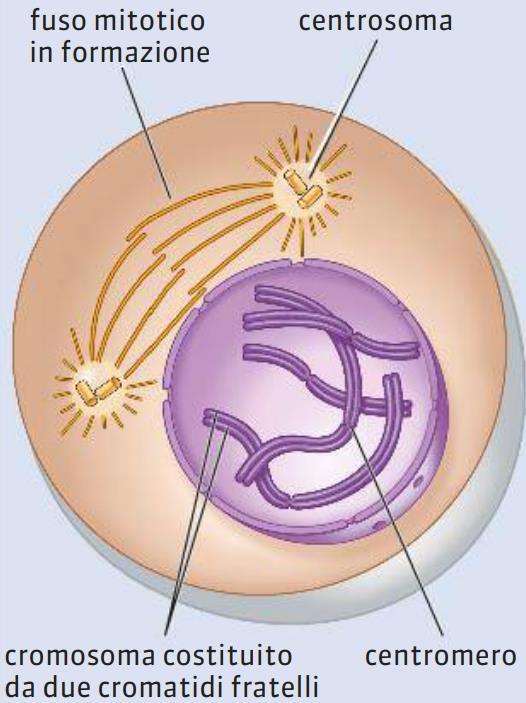
\includegraphics[width=7.5cm]{./resources/profase.jpg}
        \vspace{-1cm}
    \end{wrapfigure}

    \textbf{Profase:}
    Durante questo stadio si verificano cambiamenti sia nel nucleo sia nel citoplasma. All'interno
    del nucleo: le fibre di cromatina si spiralizzano e condensano formando cromosomi distinti,
    visibili al microscopio ottico; scompaiono i nucleoli; ciascun cromosoma duplicato è formato
    ora da due cromatidi identici uniti a livello del centromero. Nel citoplasma incomincia a
    formarsi il fuso mitotico: i microtubuli vengono rapidamente assemblati a partire dai
    centrosomi, che si allontanano l'uno dall'altro.
    \wrapfill
\end{snippet}

\begin{snippet}{prometafase-expl}
    \setlength{\intextsep}{0pt}%
    \begin{wrapfigure}{r}{8cm}
        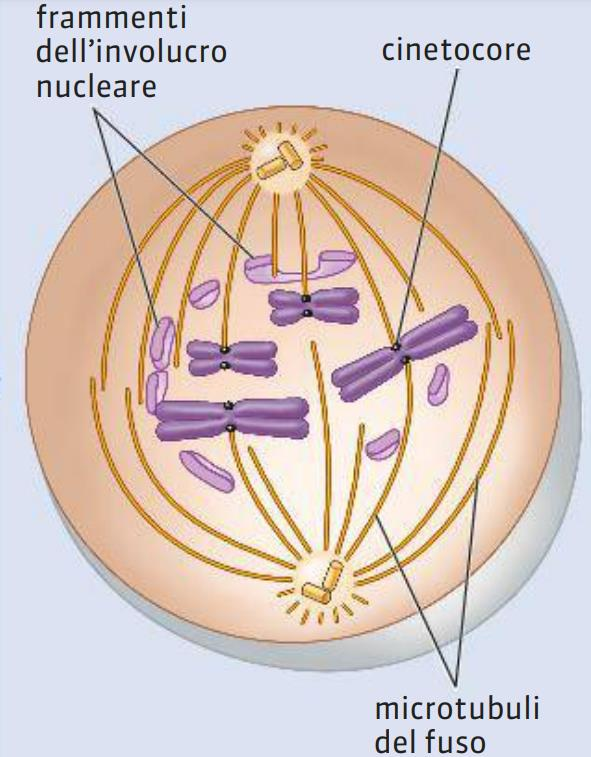
\includegraphics[width=7.5cm]{./resources/prometafase.jpg}
        \vspace{-1cm}
    \end{wrapfigure}

    \textbf{Prometafase:}
    Durante la prometafase: l'involucro nucleare si frammenta; i microtubuli raggiungono i
    cromosomi, ora molto condensati; ciascun cromatidio è unito a una struttura proteica
    chiamata cinetocore, a livello del centromero; alcuni microtubuli del fuso si attaccano ai
    cinetocori e incominciano a spostare attivamente i cromosomi; altri microtubuli del fuso
    entrano in contatto con quelli provenienti dal polo opposto. Le forze esercitate dalle proteine
    motrici associate ai microtubuli del fuso spostano i cromosomi verso il centro della cellula.
    \wrapfill
\end{snippet}

\begin{snippet}{metafase-expl}
    \setlength{\intextsep}{0pt}%
    \begin{wrapfigure}{r}{8cm}
        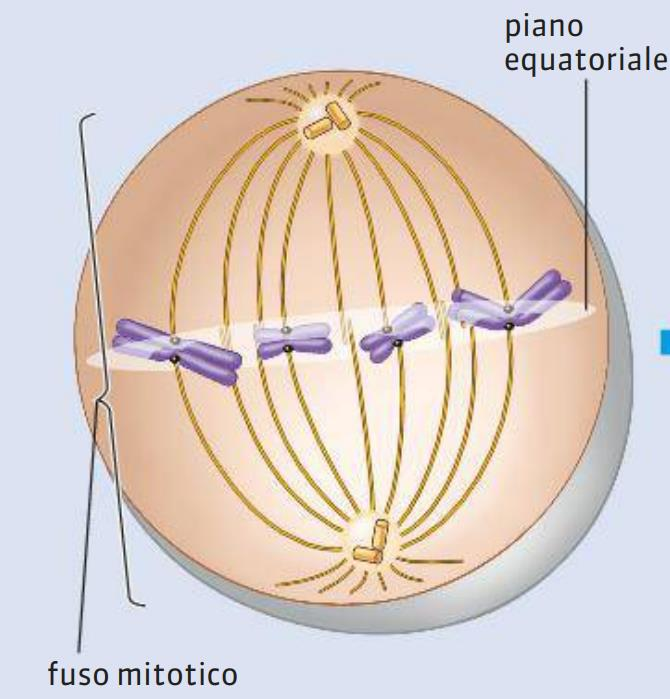
\includegraphics[width=7.5cm]{./resources/metafase.jpg}
        \vspace{-1cm}
    \end{wrapfigure}

    \textbf{Metafase:}
    È lo stadio più lungo della mitosi: il fuso mitotico è completamente formato, con i poli alle
    estremità opposte della cellula; i cromosomi si radunano in corrispondenza del piano
    equatoriale della cellula; i centromeri di tutti i cromosomi sono allineati lungo il piano
    equatoriale; per ciascun cromosoma, i cinetocori dei due cromatidi fratelli sono rivolti verso
    i poli opposti del fuso. I microtubuli attaccati a un particolare cromatidio provengono tutti da
    un polo del fuso e quelli attaccati al cromatidio fratello provengono dal polo opposto.
    \wrapfill
\end{snippet}

\begin{snippet}{Anafase-expl}
    \setlength{\intextsep}{0pt}%
    \begin{wrapfigure}{r}{8cm}
        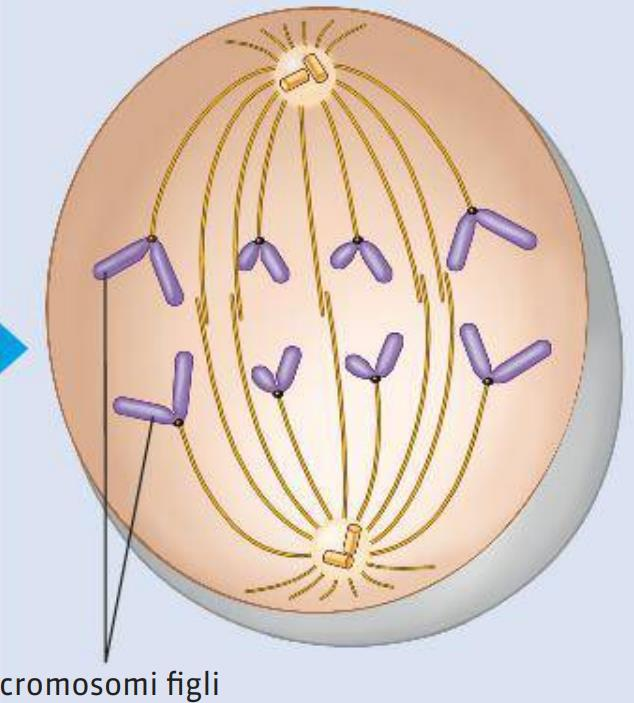
\includegraphics[width=7.5cm]{./resources/anafase.jpg}
        \vspace{-1cm}
    \end{wrapfigure}

    \textbf{Fase Anafase:}
    È lo stadio più breve della mitosi; inizia quando i due cromatidi di ciascun cromosoma si
    separano a livello del centromero e si allontanano. Ognuno dei cromatidi fratelli viene ora
    considerato un cromosoma completo. Le proteine motrici dei cinetocori, alimentate dall'ATP,
    accompagnano i cromosomi lungo i microtubuli, verso i poli opposti della cellula. Durante
    questo movimento, i microtubuli del fuso attaccati ai cinetocori si accorciano, mentre quelli
    non attaccati ai cromosomi si allungano. I poli si allontanano ulteriormente e la cellula si
    allunga. L'anafase termina quando due serie di cromosomi (equivalenti e complete) hanno
    raggiunto i poli opposti della cellula.
    \wrapfill
\end{snippet}

\begin{snippet}{telofase-expl}
    \setlength{\intextsep}{0pt}%
    \begin{wrapfigure}{r}{8cm}
        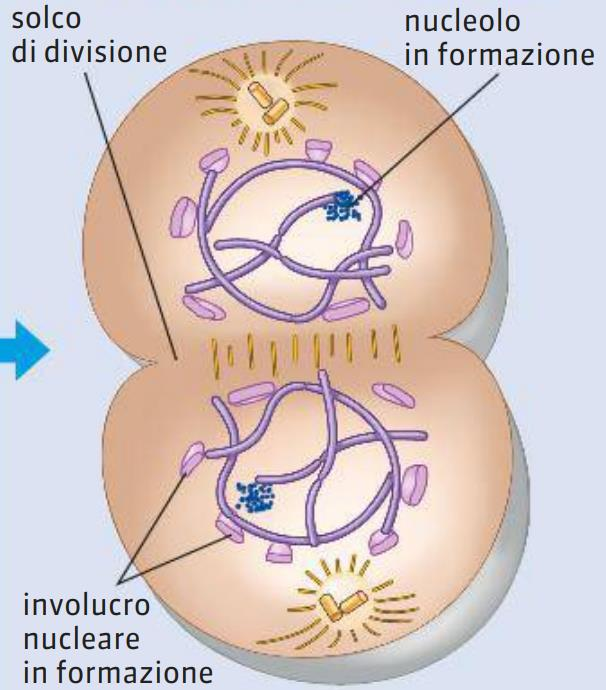
\includegraphics[width=7.5cm]{./resources/telofase.jpg}
        \vspace{-1cm}
    \end{wrapfigure}

    \textbf{Telofase:}
    È circa il processo inverso della profase: continua l'allungamento della cellula; ai due poli
    della cellula cominciano a formarsi i due nuovi nuclei; la cromatina di ciascun cromosoma
    si despiralizza e riappaiono i nucleoli; alla fine della telofase il fuso mitotico scompare e la
    mitosi, ovvero la divisione di un nucleo in due nuclei figli geneticamente identici, è terminata.
    \wrapfill
\end{snippet}

\subsubsection{Meiosi I}

\plain{I cromosomi omologhi si separano.}

\begin{snippet}{profase-i-expl}
    \setlength{\intextsep}{0pt}%
    \begin{wrapfigure}{l}{8cm}
        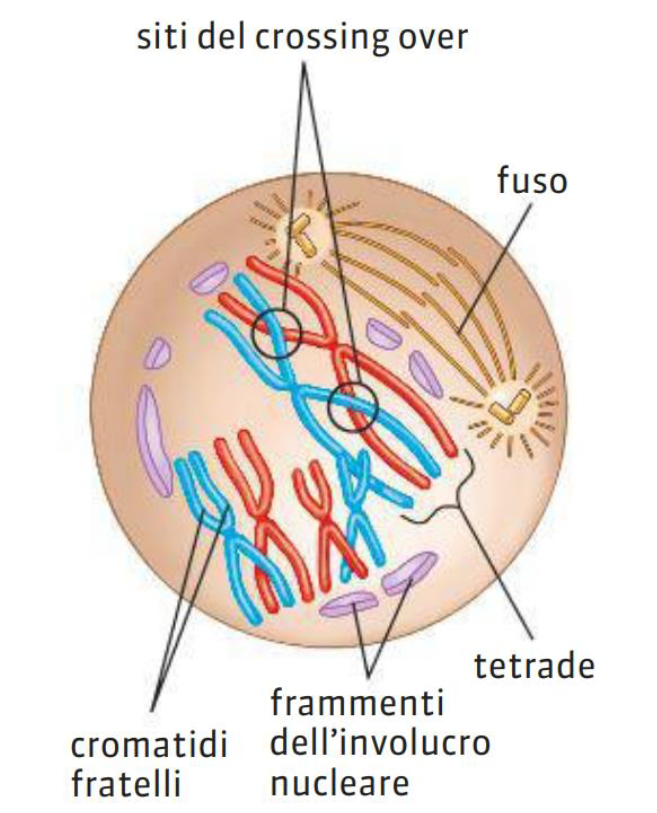
\includegraphics[width=7.5cm]{./resources/profase-i.png}
        \vspace{-1cm}
    \end{wrapfigure}

    \textbf{Profase I:}
    All'inizio di questa fase, la più complessa e lunga della meiosi, la cromatina si spiralizza e i
    cromosomi diventano visibili al microscopio. In un processo detto sinapsi, i cromosomi
    omologhi, ciascuno formato da due cromatidi fratelli, si appaiano. La struttura risultante,
    formata da quattro cromatidi, è chiamata tetrade. Durante la sinapsi, i cromatidi di
    cromosomi omologhi si scambiano segmenti di DNA in un processo, chiamato crossing over,
    che rimescola l'informazione genetica. Col procedere della profase I, i cromosomi si
    condensano sempre più. I centrosomi si allontanano l'uno dall'altro e tra di essi comincia a
    formarsi il fuso mitotico. L'involucro nucleare si frammenta e le tetradi, agganciate dai
    microtubuli del fuso, vengono trascinate verso il centro della cellula.
    \wrapfill
\end{snippet}

\begin{snippet}{metafase-i-expl}
    \setlength{\intextsep}{0pt}%
    \begin{wrapfigure}{l}{8cm}
        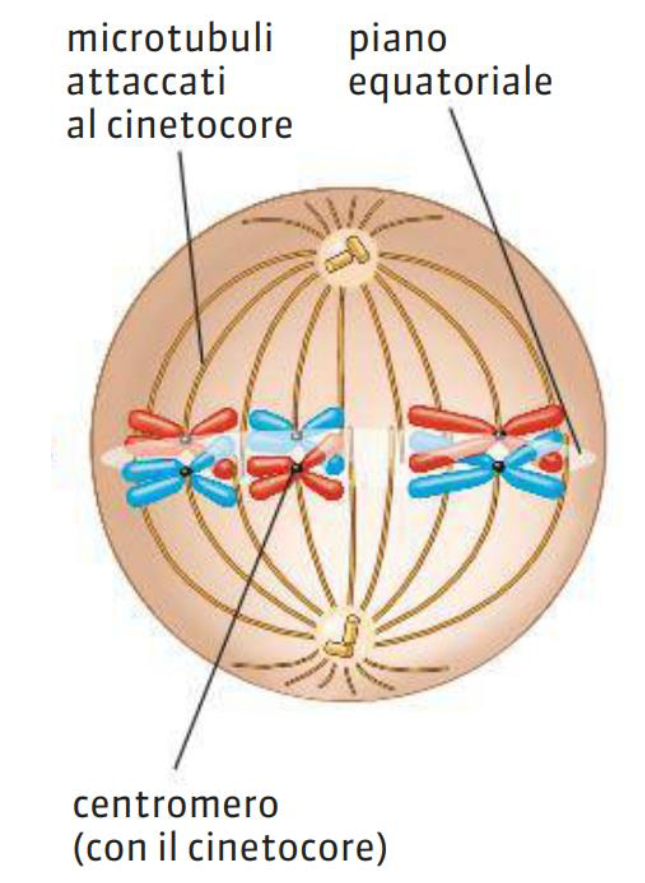
\includegraphics[width=7.5cm]{./resources/metafase-i.png}
        \vspace{-1cm}
    \end{wrapfigure}

    \textbf{Metafase I:}
    Durante la metafase I, le tetradi si allineano sul piano equatoriale della cellula. Ogni
    cromosoma è condensato e ispessito, con i cromatidi fratelli uniti in corrispondenza del
    centromero. I cromosomi sono attaccati ai microtubuli del fuso. I cromosomi omologhi di
    ogni tetrade sono uniti a microtubuli provenienti uno da un polo e l'altro dal polo opposto
    della cellula: in questo modo sono pronti a migrare verso i poli opposti della cellula.
    \wrapfill
\end{snippet}

\begin{snippet}{anafase-i-expl}
    \setlength{\intextsep}{0pt}%
    \begin{wrapfigure}{l}{8cm}
        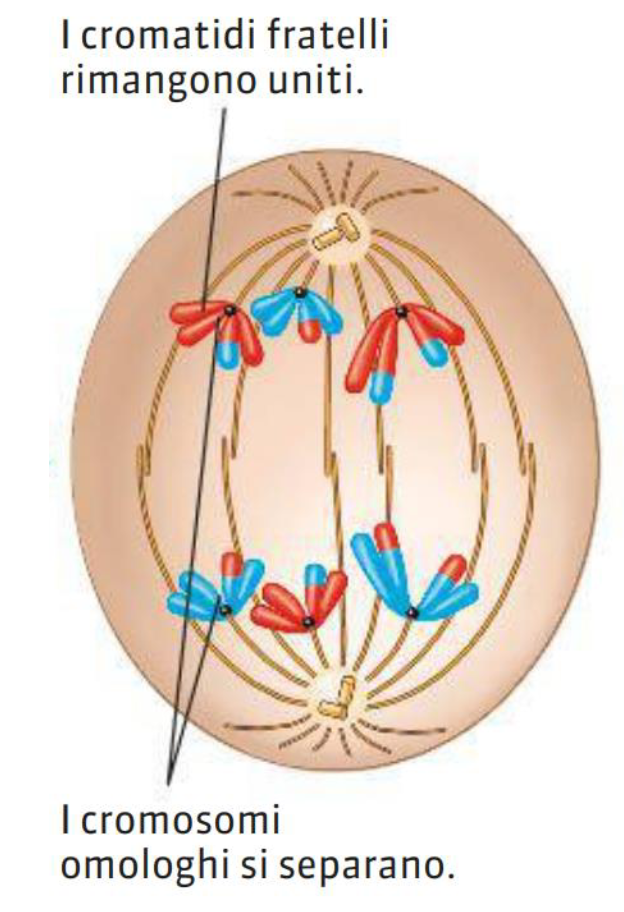
\includegraphics[width=7.5cm]{./resources/anafase-i.png}
        \vspace{-1cm}
    \end{wrapfigure}

    \textbf{Anafase I:}
    I cromosomi migrano verso i due poli della cellula. A differenza di quanto avviene nella
    mitosi, i cromatidi fratelli che costituiscono ciascun cromosoma duplicato rimangono uniti a
    livello del centromero. Soltanto le tetradi (le coppie di cromosomi omologhi) si dividono.
    \wrapfill
\end{snippet}

\begin{snippet}{telofase-i-expl}
    \setlength{\intextsep}{0pt}%
    \begin{wrapfigure}{l}{8cm}
        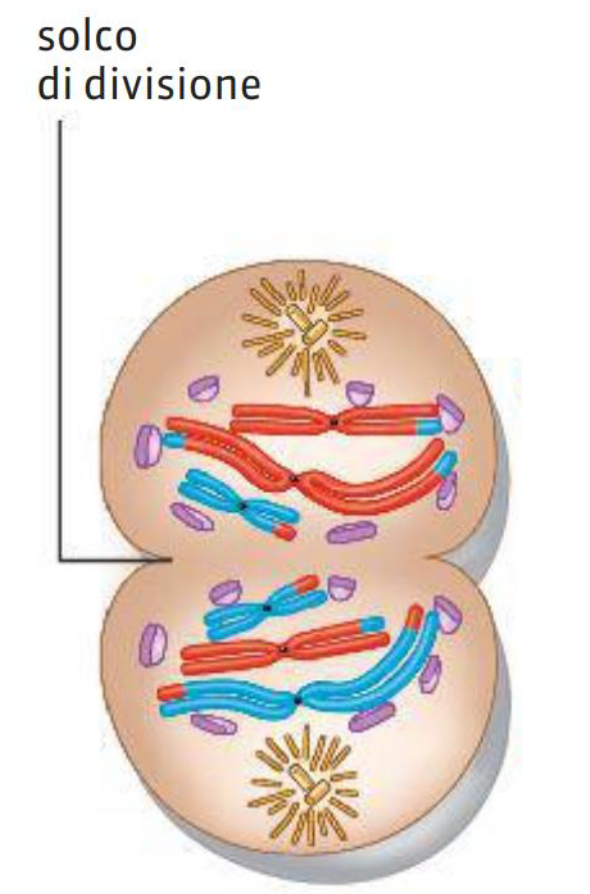
\includegraphics[width=7.5cm]{./resources/telofase-i.png}
        \vspace{-1cm}
    \end{wrapfigure}

    \textbf{Telofase e citodieresi I:}
    I cromosomi raggiungono i poli opposti della cellula. A questo punto ai due poli si trova un
    corredo cromosomico aploide, benché ogni cromosoma sia ancora costituito da due
    cromatidi fratelli. Generalmente, insieme alla telofase I avviene la citodieresi e si formano
    due cellule figlie aploidi. In alcune specie, dopo la telofase I, i cromosomi si despiralizzano,
    si riforma l'involucro nucleare e, prima che inizi la meiosi II, ha luogo un periodo di stasi. In
    altre specie le cellule figlie prodotte nella prima divisione meiotica iniziano immediatamente
    a prepararsi per la seconda divisione.
    \wrapfill
\end{snippet}

\subsubsection{Meiosi II}

\plain{I cromatidi fratelli si separano.}

\begin{snippet}{profase-ii-expl}
    \setlength{\intextsep}{0pt}%
    \begin{wrapfigure}{l}{8cm}
        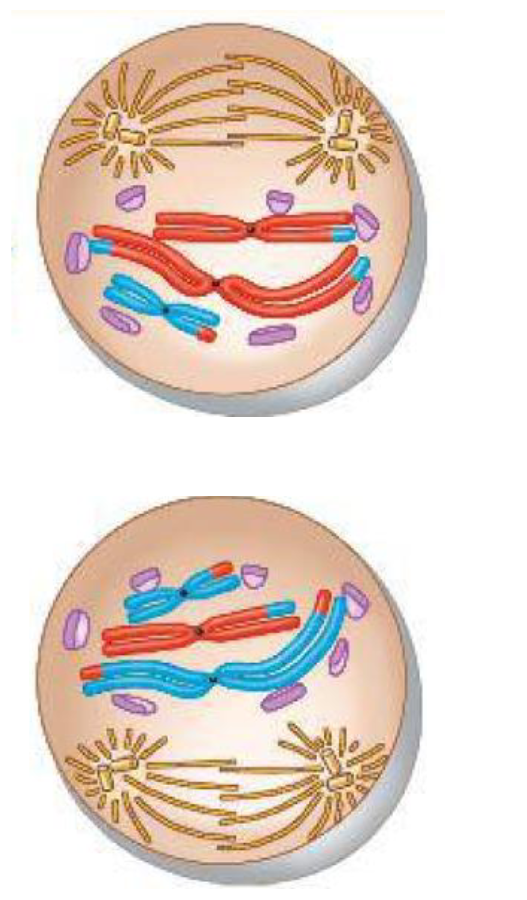
\includegraphics[width=7.5cm]{./resources/profase-ii.png}
        \vspace{-1cm}
    \end{wrapfigure}

    \textbf{Profase II:}
    Negli organismi in cui la meiosi I è seguita da una stasi, i cromosomi tornano a condensarsi
    e durante la profase II l'involucro nucleare si frammenta. Durante la profase II si forma un
    fuso che sposta i cromosomi verso il centro della cellula.
    \wrapfill
\end{snippet}

\begin{snippet}{metafase-ii-expl}
    \setlength{\intextsep}{0pt}%
    \begin{wrapfigure}{l}{8cm}
        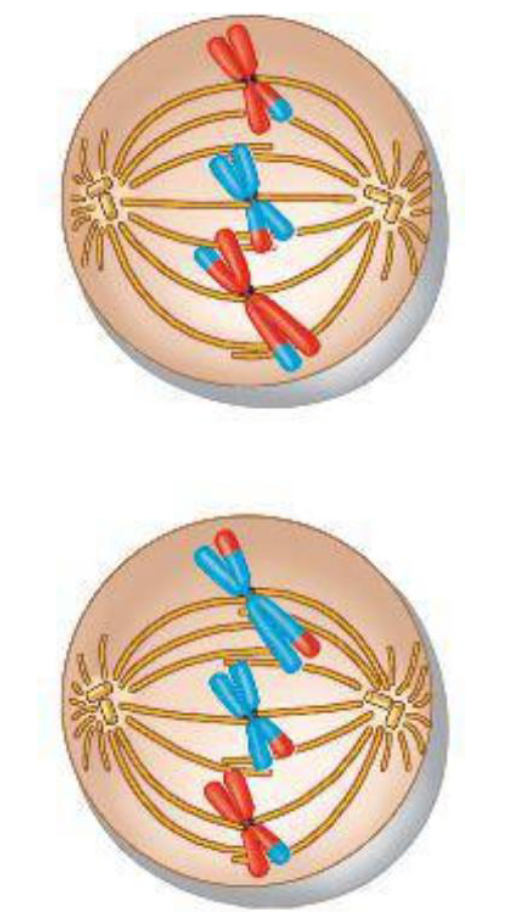
\includegraphics[width=7.5cm]{./resources/metafase-ii.png}
        \vspace{-1cm}
    \end{wrapfigure}

    \textbf{Metafase II:}
    I cromosomi si allineano sul piano equatoriale della cellula (come avviene nella mitosi) con
    i cinetocori dei cromatidi fratelli rivolti verso i poli opposti della cellula. A causa del crossing
    over, che si è verificato nella metafase I, i due cromatidi fratelli di ciascun cromosoma non
    sono identici.
    \wrapfill
\end{snippet}

\begin{snippet}{anafase-ii-expl}
    \setlength{\intextsep}{0pt}%
    \begin{wrapfigure}{l}{8cm}
        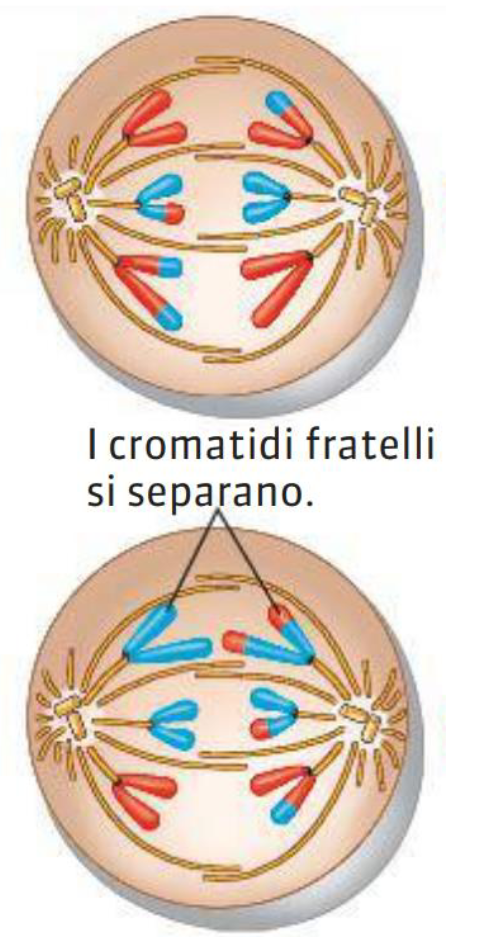
\includegraphics[width=7.5cm]{./resources/anafase-ii.png}
        \vspace{-1cm}
    \end{wrapfigure}

    \textbf{Anafase II:}
    I centromeri dei cromatidi fratelli si separano. I cromatidi fratelli di ogni coppia si spostano
    verso i poli opposti della cellula.
    \wrapfill
\end{snippet}

\begin{snippet}{telofase-ii-expl}
    \setlength{\intextsep}{0pt}%
    \begin{wrapfigure}{l}{8cm}
        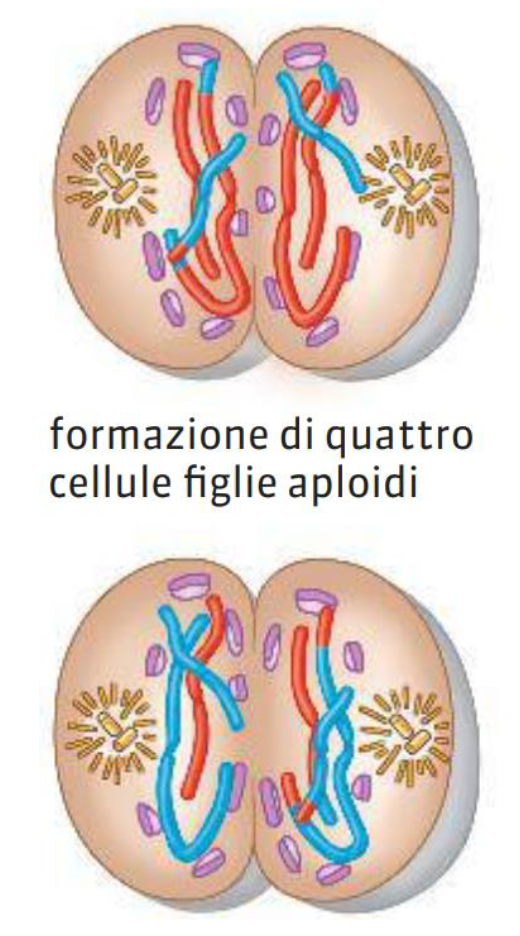
\includegraphics[width=7.5cm]{./resources/telofase-ii.png}
        \vspace{-1cm}
    \end{wrapfigure}

    \textbf{Telofase e citodieresi II:}
    Nella telofase II ai poli opposti della cellula si riformano i nuclei con le loro membrane e, allo
    stesso tempo, si verifica la citodieresi. Al termine del processo vi sono quattro cellule figlie,
    geneticamente diverse l'una dall'altra, ognuna con un corredo cromosomico aploide.
    \wrapfill
\end{snippet}

\subsection{Citodieresi}

\begin{snippetdefinition}{citodieresi-definition}{Citodieresi}
    Nella citodieresi si compie la separazione delle due cellule figlie. Di solito, la divisione del
citoplasma avviene contemporaneamente alla telofase.
\end{snippetdefinition}

\begin{snippet}{ciclo-cellulare-expl3}
    Se la cellula diviene differenziata resterà sempre in G\({}_0\).
    \\
    Il DNA, durante tutta l'interfase, è sotto forma di cromatina nel nucleo.
    Durante la fase S dell'interface, inizia la duplicazione.
    Si creano delle bolle di duplicazione sui cromosomi, formando
    coppie di cromosomi omologhi duplicati (I cromosomi omologhi sono incollati fra di loro).
    Ogni cromosoma duplicato ha due cromatidi fratelli che sono assolutamente identici.
    In mitosi abbiamo solo a che vedere con cromosomi spiralizzati.
    I due cromatidi fratelli, appena staccati, diventano cromosomi e si posizionano in cellule diverse.

    Prima della meiosi e mitosi, vi è la medesima situazione: 46 cromosomi omologhi duplicati.
    Nella metafase della mitosi, i 46 cromosomi sono uno in fila all'altro,
    mentre nella meiosi si mettono a coppie uno in fila all'altro (per cui 23 coppie in fila).

    Nella fase G1 la cellula non fa nulla e continuano la loro vita svolgendo le loro funzioni metaboliche. 
    Le cellule staminali o quelle che diventano gameti entrano nella fase S in cui il DNA viene duplicato. 
    Nella fase G2 la cellula si prepara alla divisione, e inizia a spiralizzare la cromatina. 
    Tutto ciò si chiama interfase.
    Nella fase mitotica la cellula viene divisa nella mitosi e quanto tutto è separato si taglia e si hanno due cellule separate, questa fase si chiama citodieresi.
    Nella realtà la cromatina non contiene i cromosomi spiralizzati, a differenza del disegno.

    Il ciclo della cellula è controllato in base all'ambiente esterno.
    Se la cellula è sana e vi è nutrimento, la cellula può andare in mitosi.
    Vi sono quindi tre controlli o checkpoint che bloccano il passaggio ad una fase ulteriore
    se le condizioni non sono rispettate.
    Le cellule cancerogene eludono questi checkpoint.
\end{snippet}

\includesnpt[width=45\%|src=/snippet/static/ciclo-cellulare3.png]{centered-img}

\begin{snippet}{ciclo-cellulare-punti-controllo}
    \begin{itemize}
        \item \textbf{Punto di controllo G1:}
            Punto di controllo del ciclo cellulare. La cellula entra nella fase G0 o, se il DNA è danneggiato
            in modo irreparabile, avviene l'apoptosi. Altrimenti, la cellula viene avviata alla divisione,
            proseguendo il ciclo.
        \item \textbf{Punto di controllo G2:}
            Punto di controllo della mitosi. La divisione mitotica avviene solo se il DNA è duplicato
            correttamente, altrimenti, se il DNA è danneggiato in modo irreparabile, avviene l'apoptosi.
        \item \textbf{Punto di controllo M:}
            Punto di controllo del fuso mitotico. Se i cromosomi non sono allineati correttamente lungo
            le fibre del fuso, la mitosi non procede.
    \end{itemize}
\end{snippet}

\begin{snippetdefinition}{tetrade-definition}{Tetrade}
    Nella metafase della meiosi, le coppie di cromosomi omologhi vengono chiamate
    \textit{tetradi}.
\end{snippetdefinition}

\includesnpt[width=67\%|src=/snippet/static/meiosi-schema.png]{centered-img}

% Schema MITOSI / MEIOSI giallo e violaceo
% Meglio "duplicazione del materiale genetico" al posto di "duplicazione dei cromosomi"

\end{document}